%!TEX root = ../../report.tex

\subsubsection{Noise} % (fold)
\label{ssub:noise}


``To generate irregular procedural textures, we need an irregular primitive function, usually called noise" \cite{Ebert2002}. It's a pseudorandom function that gave the goal to break the monotony of a pattern and make it look more random.
Perlin Noise is the most known and used noise function. It was created by Ken Perlin, for the movie Tron 1982 with the aiming to generate natural looking textures.

The psedorandom property is important and a true random function like \emph{white noise} would not do the job. If we generate a texture based on white noise the pattern would change every time it's generated and we would like that the it stays the same, frame after frame. This is achieved with the use of inputs for this functions that with the same input returns always the same output sequence. 

The properties of an ideal \emph{noise} functions are as follows \cite{Ebert2002}:
\begin{itemize}
	\item \emph{noise} is a repeatable pseudorandomm function of its inputs
	\item \emph{noise} has a known range, namely, from -1 to 1.
	\item \emph{noise} is band-limited, with a maximum frequency of about 1.
	\item \emph{noise} doesn't exhibit obvious periodicities or regular patterns. Such pseudorandom functions are always periodic, but the period can be made very long and therefore the periodicity is not conspicuous.
	\item \emph{noise} is \emph{stationary} - that is, its statistical character should be translationally invariant
	\item \emph{noise} is \emph{isotropic} - that is, its statistical character should be rotationally invariant
\end{itemize}

With this noise function, it's generated a sequence of values that are interpolated to generate a coherent noise. With the application of \emph{turbulence} that is composition of several layers of this noise with different frequencies and amplitudes forming a coherent noise. This layers are called \emph{Octaves} and the ratio between amplitude and frequency of the layers can be expressed as a constant known as \emph{persistence} \cite{Kelly2008}. With the result we can create a texture that looks natural and with fractal like structure.


\begin{figure}[H]
	\centering
	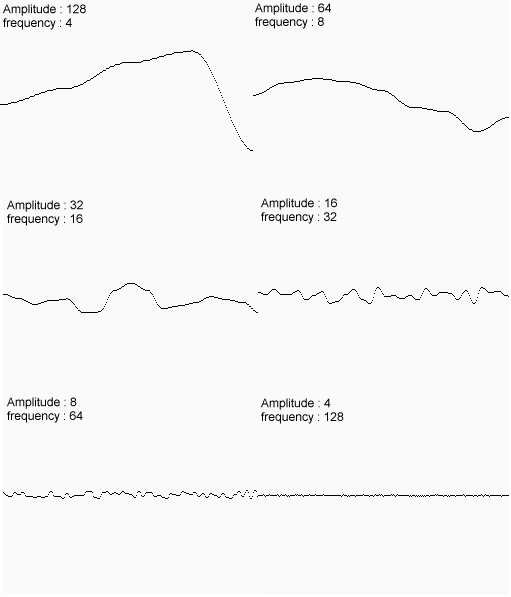
\includegraphics[width=0.75\textwidth]{img/Theory/Perlin_Noise/Merge.png}
	\caption{Different noise functions}
	\label{fig:merge}
\end{figure}



For instance, the Figure~\ref{fig:merge} shows the result of the interpolation over six noise functions with different frequencies and different amplitudes. And the sum of all this functions is the exibithed in the Figure~\ref{fig:noise} \cite{NoisesELIAS}.

\begin{figure}[htbp]
	\centering
	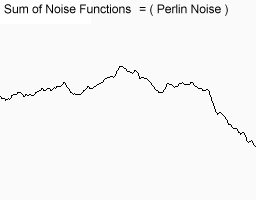
\includegraphics[width=0.65\textwidth]{img/Theory/Perlin_Noise/perlin1.png}
	\caption{``You may even imagine that it looks a little like a mountain range."}
	\label{fig:noise}
\end{figure}

Noise is also used to 

% subsubsection noise (end)
